\section{UML}
\subsection{Introduction}
As seen in the previous sections, the requirements document is very important, as any mistake, ambiguity,
or misunderstanding of the client's needs can lead to a project restart. We've reviewed the high-level
structure of a requirements document; one of the most important parts is the functional requirements, which can
be expressed in natural language. This approach is easy to implement and understand but isn't very precise, doesn't
automate verification, and relies solely on the linguistic experience of the writer. There is also a formal approach
based on mathematical theory, which automates verification, is very precise, but is hard to master and 
time-consuming. Finally, there is a semi-formal approach that benefits from the advantages of both natural and 
formal language; an example of this is UML (Unified Modeling Language).
\subsection{UML(Unified Modeling Language)}
UML is a semi-formal language that is easy to understand and widely used by developers. It divides into two main categories of diagrams:
\begin{itemize}
    \item Structure Diagram : Represent the static aspects of a system, showing its classes, objects, and relationships. 
    \item Behaviour Diagram :  Describes the dynamic aspects of a system, illustrating how actors interact with the system and how the system changes over time.
\end{itemize}
In this section we will focus on Use case diagram
\begin{center}
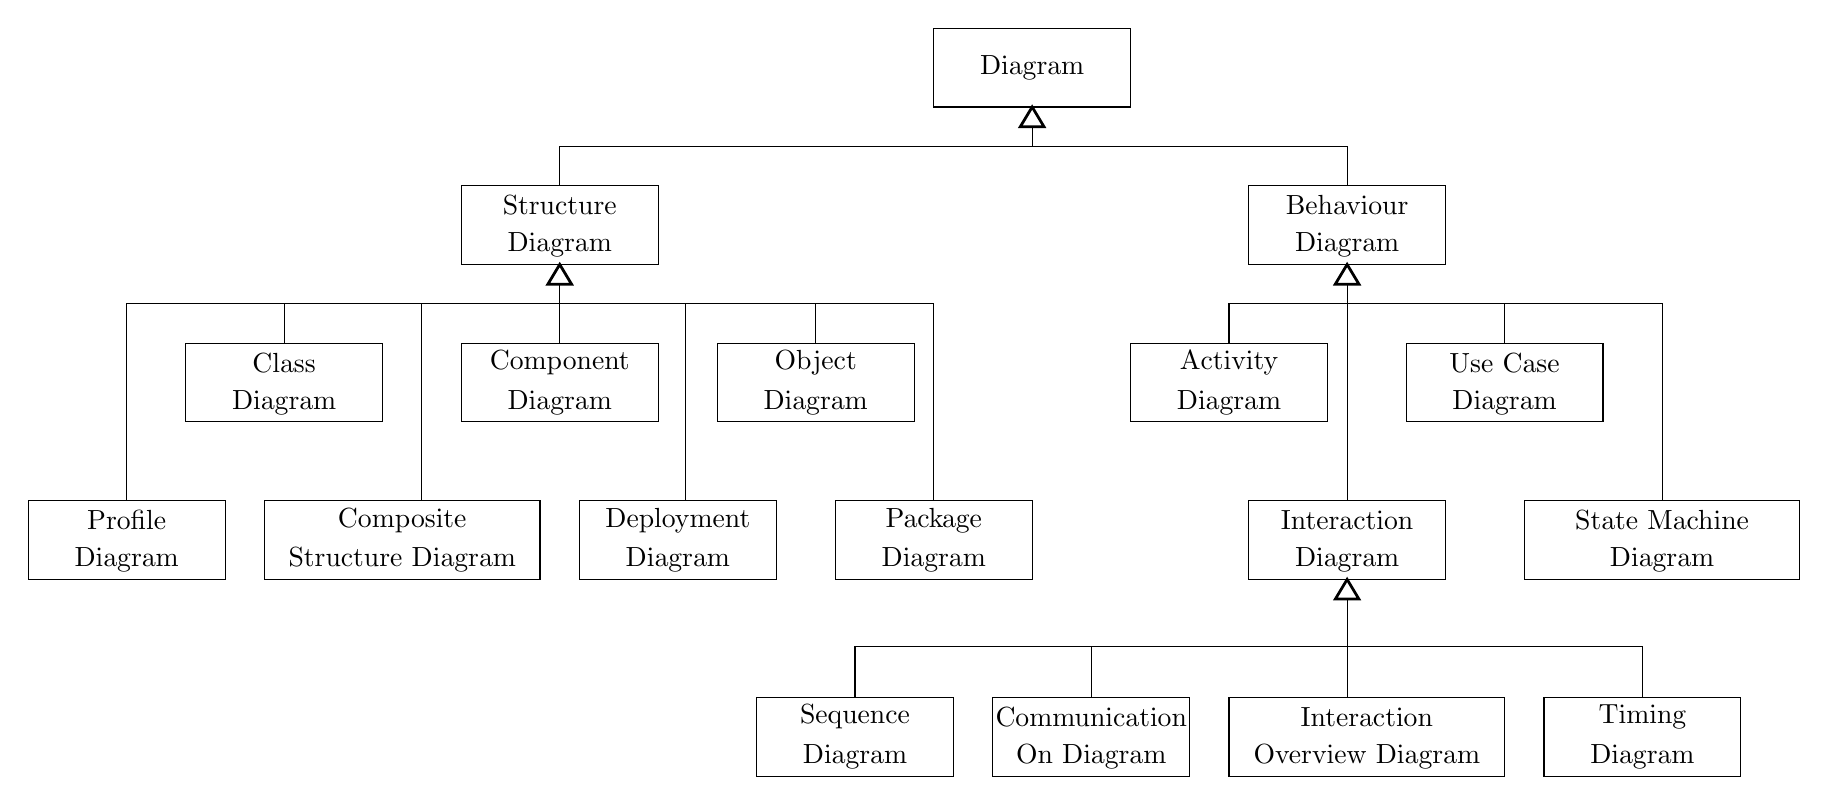
\begin{tikzpicture}
    \draw(0,0) rectangle(2.5,1);
    \node at(1.25,0.5) {Diagram};
    
    \coordinate (A) at (1.25,0);  
    \coordinate (B) at (1.1,-0.25);  
    \coordinate (C) at (1.4,-0.25);
    \draw[line width=1pt] (A) -- (B) -- (C) -- cycle;
    
    \draw (1.25,-0.25) -- (1.25,-0.5);
    \draw (-4.75,-1) -- (-4.75,-0.5) -- (5.25,-0.5) -- (5.25,-1);

    \draw(-6,-2) rectangle(-3.5,-1);
    \node at (-4.75,-1.25){Structure};
    \node at (-4.75,-1.75){Diagram};
   
    \coordinate (A) at (-4.75,-2);  
    \coordinate (B) at (-4.9,-2.25);  
    \coordinate (C) at (-4.6,-2.25);
    \draw[line width=1pt] (A) -- (B) -- (C) -- cycle;
   
    \draw (-4.75,-2.25) -- (-4.75,-3);
    \draw (-10.25,-5) -- (-10.25,-2.5) -- (0,-2.5) -- (0,-5);

    \draw (-6,-4) rectangle(-3.5,-3);
    \node at (-4.75,-3.25){Component};
    \node at (-4.75,-3.75){Diagram};
    \draw (-4.75,-3) -- (-4.75,-2.5);
    
    \draw (-9.5,-4) rectangle(-7,-3);
    \node at (-8.25,-3.25){Class};
    \node at (-8.25,-3.75){Diagram};
    \draw (-8.25,-3) -- (-8.25,-2.5);
 
    \draw (-2.75,-4) rectangle(-0.25,-3);
    \node at (-1.5,-3.25){Object};
    \node at (-1.5,-3.75){Diagram};
    \draw (-1.5,-3) -- (-1.5,-2.5);
    
    \draw (-11.5,-6) rectangle(-9,-5);
    \node at (-10.25,-5.25){Profile};
    \node at (-10.25,-5.75){Diagram};
    
    \draw (-8.5,-6) rectangle(-5,-5);
    \node at (-6.75,-5.25){Composite};
    \node at (-6.75,-5.75){Structure Diagram};
    \draw (-6.5,-5) -- (-6.5,-2.5);

    \draw (-4.5,-6) rectangle(-2,-5);
    \node at (-3.25,-5.25){Deployment};
    \node at (-3.25,-5.75){Diagram};
    \draw (-3.15,-5) -- (-3.15,-2.5);
    
    \draw (-1.25,-6) rectangle(1.25,-5);
    \node at (0,-5.25){Package};
    \node at (0,-5.75){Diagram};

    \draw(4,-2) rectangle(6.5,-1);
    \node at (5.25,-1.25){Behaviour};
    \node at (5.25,-1.75){Diagram};

    \coordinate (A) at (5.25,-2);  
    \coordinate (B) at (5.1,-2.25);  
    \coordinate (C) at (5.4,-2.25);
    \draw[line width=1pt] (A) -- (B) -- (C) -- cycle;
    
    \draw (2.5,-4) rectangle(5,-3);
    \node at (3.75,-3.25){Activity};
    \node at (3.75,-3.75){Diagram};
   
    \draw  (3.75,-3)--(3.75,-2.5)--(9.25,-2.5)--(9.25,-5);

    \draw (6,-4) rectangle(8.5,-3);
    \node at (7.25,-3.25){Use Case};
    \node at (7.25,-3.75){Diagram};
    \draw  (7.25,-3)--(7.25,-2.5);

    \draw (4,-6) rectangle(6.5,-5);
    \node at (5.25,-5.25){Interaction};
    \node at (5.25,-5.75){Diagram};
    \draw  (5.25,-5)--(5.25,-2.25);
    
    \coordinate (A) at (5.25,-6);  
    \coordinate (B) at (5.1,-6.25);  
    \coordinate (C) at (5.4,-6.25);
    \draw[line width=1pt] (A) -- (B) -- (C) -- cycle;
    
    \draw (7.5,-6) rectangle(11,-5);
    \node at (9.25,-5.25){State Machine};
    \node at (9.25,-5.75){Diagram};

    \draw (3.75,-8.5) rectangle(7.25,-7.5);
    \node at (5.5,-7.75){Interaction};
    \node at (5.5,-8.25){Overview Diagram};
    \draw  (5.25,-7.5)--(5.25,-6.25);
    
    \draw (7.75,-8.5) rectangle(10.25,-7.5);
    \node at (9,-7.75){Timing};
    \node at (9,-8.25){Diagram};

    \draw (0.75,-8.5) rectangle(3.25,-7.5);
    \node at (2,-7.75){Communication};
    \node at (2,-8.25){On Diagram};
    \draw  (2,-7.5)--(2,-6.85);
    
    \draw (-2.25,-8.5) rectangle(0.25,-7.5);
    \node at (-1,-7.75){Sequence};
    \node at (-1,-8.25){Diagram};

    \draw (-1,-7.5)--(-1,-6.85)--(9,-6.85)--(9,-7.5);
\end{tikzpicture}
\end{center}
\vspace{2cm}


\subsection{Use Case Diagram}
A use case diagram is a graphical representation of a behavior diagram, composed of three main elements:

\begin{itemize} 
    \item Actors: Actors represent roles that interact with the system. Each actor performs a set of 
actions called use cases, which represent features of the software they interact with. Actors are
depicted as stick figures and can be either human or non-human.
   \begin{itemize}
    \item Human actors: Individuals using the system.
    \item Non-human actors: Entities such as hardware (e.g., sensors, cameras) 
     or software (e.g., APIs, dependencies). 
   \end{itemize}
   \item Use Cases (Features): These represent features or functions of the software and are shown as ellipses , they have to be programmable.
   \item Associations: Associations are the connections between actors and use cases, depicted as lines. These lines 
indicate what action (use case) each actor can perform. 
\end{itemize}

\vspace{0.5cm}
\subsubsection*{\underline{Example:}}

\vspace{0.5cm}
\begin{center}
    \begin{tikzpicture}

        \draw[->, red] (-6.25,-1.75) -- (-4.5,-1.75);
        \node at (-7,-1.65){\textcolor{red}{Actor}};
        \draw[->, red] (-5.75,-3.5) -- (-3.25,-3.5);
        \node at (-6.75,-3.45){\textcolor{red}{Association}};
        \draw[<-,red] (2.65,0) -- (5,0);
        \node at (5.75,0.07){\textcolor{red}{Use Case}};
        
        \fill[MyBlue] (-4,-1.5) circle(0.15);
        \draw (-4,-1.5) circle(0.15);
        \draw (-4,-1.65)--(-4,-2);
        \draw (-4.25,-1.795)--(-3.75,-1.795);
        \draw (-4,-2) -- (-3.75,-2.25);
        \draw (-4,-2) -- (-4.25,-2.25);
        \node at (-3.995,-2.35){\tiny Customer};

        \draw (-3.75,-1.35) -- (-2.5,0);
        \fill[MyBlue] (0,0) ellipse (2.5 and 0.5);
        \draw (0,0) ellipse (2.5 and 0.5);
        \node at(0.08,0){View Billing Statements};


        \draw (-3.5,-2) -- (-2.5,-2);
        \fill[MyBlue] (0,-2) ellipse (2.5 and 0.5);
        \draw (0,-2) ellipse (2.5 and 0.5);
        \node at(0.08,-2){Place Order};


        \draw (-3.75,-2.75) -- (-2.5,-4);
        \fill[MyBlue] (0,-4) ellipse (2.5 and 0.5);
        \draw (0,-4) ellipse (2.5 and 0.5);
        \node at(0.08,-4){Cancel Order};

        \fill[MyBlue] (-4,-5.5) circle(0.15);
        \draw (-4,-5.5) circle(0.15);
        \draw (-4,-5.65)--(-4,-6);
        \draw (-4.25,-5.795)--(-3.75,-5.795);
        \draw (-4,-6) -- (-3.75,-6.25);
        \draw (-4,-6) -- (-4.25,-6.25);
        \node at (-3.995,-6.35){\tiny Customer Service Assistant};
        
        \fill[MyBlue] (0.5,-6) ellipse (2.5 and 0.5);
        \draw (0.5,-6) ellipse (2.5 and 0.5);
        \draw (-3.5,-6) -- (-2,-6);
        \node at(0.58,-6){Create Customer Order};
 
        \fill[MyBlue] (11,-5.5) circle(0.15);
        \draw (11,-5.5) circle(0.15);
        \draw (11,-5.65)--(11,-6);
        \draw (10.75,-5.795)--(11.25,-5.795);
        \draw (11,-6) -- (11.25,-6.25);
        \draw (11,-6) -- (10.75,-6.25);
        \node at (10.995,-6.35){\tiny Regional Manager};
       

        \draw (9,-6) -- (10.5,-6);
        \fill[MyBlue] (6.5,-6) ellipse (2.5 and 0.5);
        \draw (6.5,-6) ellipse (2.5 and 0.5);
        \node at(6.58,-6){Generate Statistic Report};


        \draw (9,-4) -- (10.5,-4);
        \fill[MyBlue] (6.5,-4) ellipse (2.5 and 0.5);
        \draw (6.5,-4) ellipse (2.5 and 0.5);
        \node at(6.58,-4){Arrange Delivery};


        \draw (9,-2) -- (10.5,-3.25);
        \fill[MyBlue] (6.5,-2) ellipse (2.5 and 0.5);
        \draw (6.5,-2) ellipse (2.5 and 0.5);
        \node at(6.58,-2){Print Logistic Report};

        \fill[MyBlue] (11,-3.5) circle(0.15);
        \draw (11,-3.5) circle(0.15);
        \draw (11,-3.65)--(11,-4);
        \draw (10.75,-3.795)--(11.25,-3.795);
        \draw (11,-4) -- (11.25,-4.25);
        \draw (11,-4) -- (10.75,-4.25);

        \node at (10.995,-4.35){\tiny Logistic Departement Manager};

    \end{tikzpicture}
\end{center}

\vspace{1cm}
\begin{prettyBox}{Internal \& External Actors }{red}

In a use case diagram all actors have to be internal to the software and all use cases must be
features from the software that are programmable
\begin{itemize}
    \item Internal Actor : must interact with the software 
    \item External Actor : don't interact with the software
\end{itemize}

\end{prettyBox}

\begin{prettyBox}{The Ideal Level Of Decomposition Of Use Cases}{red}

In a use case diagram, the level of decomposition for use cases should strike a balance. It shouldn’t
be too specific, as this can make the diagram cluttered and difficult to read, nor too generic, which
can make it hard to understand. A moderate level of detail is ideal.

\vspace{0.15cm}
It's acceptable to leave some use cases at a more generic level without decomposing them, especially
since the diagram is accompanied by a document that provides detailed explanations. 
This document defines and elaborates on all sub-use cases as needed.

\end{prettyBox}

\vspace{1cm}
\subsubsection{Relations In Use Case Diagram}
\begin{itemize}
    \item  \textbf{Generalization}:  Generalization establishes a hierarchical relationship that helps organize
actors and use cases in UML diagrams. 
        \begin{itemize}
            \item  \textbf{Between Actors}: When a child actor is linked to a parent actor, it inherits all the roles and
responsibilities of the parent actor,in addition to its own specific roles. This helps clarify who can perform
what actions in the system.

\vspace{0.35cm}
\begin{center}
       \begin{tikzpicture}
        \fill[MyBlue] (-4,-1.5) circle(0.15);
        \draw (-4,-1.5) circle(0.15);
        \draw (-4,-1.65)--(-4,-2);
        \draw (-4.25,-1.795)--(-3.75,-1.795);
        \draw (-4,-2) -- (-3.75,-2.25);
        \draw (-4,-2) -- (-4.25,-2.25);
   

        \coordinate (A) at (-4,-2.25);  
        \coordinate (B) at (-4.15,-2.5);  
        \coordinate (C) at (-3.85,-2.5);
        \draw[line width=1pt] (A) -- (B) -- (C) -- cycle;

        \fill[MyBlue] (-4,-3.15) circle(0.15);
        \draw (-4,-3.15) circle(0.15);
        \draw (-4,-3.3)--(-4,-3.65);
        \draw (-4.25,-3.445)--(-3.75,-3.445);
        \draw (-4,-3.65) -- (-3.75,-3.9);
        \draw (-4,-3.65) -- (-4.25,-3.9); 

        \fill[MyBlue] (-7,-3.15) circle(0.15);
        \draw (-7,-3.15) circle(0.15);
        \draw (-7,-3.3)--(-7,-3.65);
        \draw (-7.25,-3.445)--(-6.75,-3.445);
        \draw (-7,-3.65) -- (-6.75,-3.9);
        \draw (-7,-3.65) -- (-7.25,-3.9);

        \fill[MyBlue] (-1,-3.15) circle(0.15);
        \draw (-1,-3.15) circle(0.15);
        \draw (-1,-3.3)--(-1,-3.65);
        \draw (-1.25,-3.445)--(-0.75,-3.445);
        \draw (-1,-3.65) -- (-0.75,-3.9);
        \draw (-1,-3.65) -- (-1.25,-3.9);

        \draw (-7,-2.85)--(-7,-2.65) -- (-1,-2.65) -- (-1,-2.85);
        \draw (-4,-2.5)--(-4,-2.85);

    \end{tikzpicture} 
\end{center}


\vspace{0.35cm}

            \item  \textbf{Between Use Cases}: Allows a feature to be divided into multiple, more specific
versions. These child use cases represent the same general feature but can differ in their implementation or method.
This promotes reusability and clarity in how features are handled in different scenarios.
        \end{itemize}

\vspace{0.35cm}
        \begin{center}
            \begin{tikzpicture}
            \fill[MyBlue] (0,0) ellipse (2.5 and 0.5);
            \draw (0,0) ellipse (2.5 and 0.5);
            \node at (0.08,0) {Parent User Case};
        
        \coordinate (A) at (0,-0.5);  
        \coordinate (B) at (-0.15,-0.75);  
        \coordinate (C) at (0.15,-0.75);
        \draw[line width=1pt] (A) -- (B) -- (C) -- cycle;
        
           \fill[MyBlue] (0,-2) ellipse (2.5 and 0.5);
            \draw (0,-2) ellipse (2.5 and 0.5);
            \node at (0.08,-2) {child User Case 2};
            
            \fill[MyBlue] (7,-2) ellipse (2.5 and 0.5);
            \draw (7,-2) ellipse (2.5 and 0.5);
            \node at (7.08,-2) {child User Case 3};

            \fill[MyBlue] (-7,-2) ellipse (2.5 and 0.5);
            \draw (-7,-2) ellipse (2.5 and 0.5);
            \node at (-6.92,-2) {child User Case 1};

            \draw (-7,-1.5) -- (-7,-1) -- (7,-1) -- (7,-1.5);
            \draw (0,-1.5) -- (0,-0.75);
            \end{tikzpicture}
        \end{center}
          

\vspace{0.35cm}

    \item  \textbf{Inclusion}: This relationship applies only between use cases. The destination use case 
must execute before  the source use case whenever the source use case is invoked. 
 
\vspace{0.35cm}
        \begin{center}
            \begin{tikzpicture}
                
            \fill[MyBlue] (-2,0) ellipse (2.5 and 0.5);
            \draw (-2,0) ellipse (2.5 and 0.5);
            \node at (-1.92,0){Source};
            
            \draw[->] (0.5,0)--(4,0);
            \node at (2.25,0.25){"include"};

            \fill[MyBlue] (6.5,0) ellipse (2.5 and 0.5);
            \draw (6.5,0) ellipse (2.5 and 0.5);
            \node at (6.58,0){Destination};
            \end{tikzpicture}
    \end{center}
    

\vspace{0.35cm}
\item  \textbf{Extension}: This relationship applies only between use cases. Before executing the destination use case, 
a specific condition is checked. If the condition is met, the source use case will execute
before the destination use case.
 
\vspace{0.35cm}
\begin{center}
            \begin{tikzpicture}
                
            \fill[MyBlue] (-2,0) ellipse (2.5 and 0.5);
            \draw (-2,0) ellipse (2.5 and 0.5);
            \node at (-1.92,0){Source};
            
            \draw[->] (0.5,0)--(4,0);
            \node at (2.25,0.25){"extend"};

            \fill[MyBlue] (6.5,0) ellipse (2.5 and 0.5);
            \draw (6.5,0) ellipse (2.5 and 0.5);
            \node at (6.58,0){Destination};
            \end{tikzpicture}
    \end{center}

\end{itemize}


\subsubsection*{\underline{Example:}}
Let's Take the example of a bank application\\\\ 
\textbf{\underline{Generalisation Between Use Cases:}}

\vspace{0.25cm}
the diagram below shows a generalisation relationship between use case 
where the main feature is transfert that is divided into specific method and way of achieving the transfert (ATM,Manual,Online)
\vspace{0.5cm}
\begin{center}
            \begin{tikzpicture}
            \fill[MyBlue] (0,0) ellipse (2.5 and 0.5);
            \draw (0,0) ellipse (2.5 and 0.5);
            \node at (0.08,0) {Transfer};
        
        \coordinate (A) at (0,-0.5);  
        \coordinate (B) at (-0.15,-0.75);  
        \coordinate (C) at (0.15,-0.75);
        \draw[line width=1pt] (A) -- (B) -- (C) -- cycle;
        
           \fill[MyBlue] (0,-2) ellipse (2.5 and 0.5);
            \draw (0,-2) ellipse (2.5 and 0.5);
            \node at (0.08,-2) {Online transfer};
            
            \fill[MyBlue] (7,-2) ellipse (2.5 and 0.5);
            \draw (7,-2) ellipse (2.5 and 0.5);
            \node at (7.08,-2) {ATM transfer};

            \fill[MyBlue] (-7,-2) ellipse (2.5 and 0.5);
            \draw (-7,-2) ellipse (2.5 and 0.5);
            \node at (-6.92,-2) {Manual transfer};

            \draw (-7,-1.5) -- (-7,-1) -- (7,-1) -- (7,-1.5);
            \draw (0,-1.5) -- (0,-0.75);
            \end{tikzpicture}
        \end{center}


        \vspace{1cm}

\textbf{\underline{Generalisation Between Actors:}}

\vspace{0.25cm}
the diagram below shows a generalisation relationship between Actors where the child actor Service Manager 
is inheriting all roles of the parent actor teller + his own roles

\vspace{0.15cm}

\begin{center}
       \begin{tikzpicture}
        \fill[MyBlue] (-4,-1.5) circle(0.15);
        \draw (-4,-1.5) circle(0.15);
        \draw (-4,-1.65)--(-4,-2);
        \draw (-4.25,-1.795)--(-3.75,-1.795);
        \draw (-4,-2) -- (-3.75,-2.25);
        \draw (-4,-2) -- (-4.25,-2.25);
        \node at (-3,-2){Teller};


        \coordinate (A) at (-4,-2.25);  
        \coordinate (B) at (-4.15,-2.5);  
        \coordinate (C) at (-3.85,-2.5);
        \draw[line width=1pt] (A) -- (B) -- (C) -- cycle;

        \fill[MyBlue] (-4,-3.15) circle(0.15);
        \draw (-4,-3.15) circle(0.15);
        \draw (-4,-3.3)--(-4,-3.65);
        \draw (-4.25,-3.445)--(-3.75,-3.445);
        \draw (-4,-3.65) -- (-3.75,-3.9);
        \draw (-4,-3.65) -- (-4.25,-3.9); 
        \node at (-2.25,-3.65){Service Manager};
        
        \draw (-4,-2.5)--(-4,-2.85);
    \end{tikzpicture}
\end{center}

        \vspace{1cm}
\textbf{\underline{inclusion Between Use Cases:}}

\vspace{0.25cm}
the diagram below shows an inclusion relationship between use cases where each time the transfert case is invoked
the identification case must execute first 

\vspace{0.15cm}

        \begin{center}
            \begin{tikzpicture}
                
            \fill[MyBlue] (-2,0) ellipse (2.5 and 0.5);
            \draw (-2,0) ellipse (2.5 and 0.5);
            \node at (-1.92,0){Transfert};
            
            \draw[->] (0.5,0)--(4,0);
            \node at (2.25,0.25){"include"};

            \fill[MyBlue] (6.5,0) ellipse (2.5 and 0.5);
            \draw (6.5,0) ellipse (2.5 and 0.5);
            \node at (6.58,0){Identification};
            \end{tikzpicture}
    \end{center}

        \vspace{1cm}
        \newpage
\textbf{\underline{Extension Between Use Cases:}}

\vspace{0.25cm}
the diagram below shows an extension relationship between use cases where each time the transfert case is invoked
the balance check case will be executed if the value is \textgreater= 10000 DA

\vspace{0.15cm}


        \begin{center}
            \begin{tikzpicture}
                
            \fill[MyBlue] (-2,0) ellipse (2.5 and 0.5);
            \draw (-2,0) ellipse (2.5 and 0.5);
            \node at (-1.92,0){Balance Check};
            
            \draw[->] (0.5,0)--(4,0);
            \node at (2.25,0.25){"extend"};

            \fill[MyBlue] (6.5,0) ellipse (2.5 and 0.5);
            \draw (6.5,0) ellipse (2.5 and 0.5);
            \node at (6.58,0){Transfert};

            \draw (0.5,-2.25) rectangle (3.95,-1);
            \node at (2.225,-1.625){If value \textgreater=10000DA};
            \draw (2.225,-1) -- (2.225,-0.15);
            \end{tikzpicture}
    \end{center}

        \vspace{1cm}

\begin{prettyBox}{Difference Between Inclusion \& Extension}{red}

In The inclusion relation the Destination case will always execute before source case in all cases , whereas
in the extension relation the source case will execute before destination source only if certain conditions
are met

\end{prettyBox}


\vspace{0.5cm}

\begin{prettyBox}{Extends With No Conditions}{red}
If an extend relation doesn't have an explicit condition it just means that it's an option and
the actor can decide wether to trigger the extended use case or not (option)
\end{prettyBox}

\subsection{Class Diagram}

\begin{prettyBox}{What's a Class Diagram}{mypur}
A Class Diagram is a graphical representation of a structure diagram that illustrates classes, their attributes, and the relationships between them. It consists of three main components:
\begin{itemize}
    \item \textbf{UML Elements}: Classes , enumeration , interfaces.
    \item \textbf{Relations}: Connections that define how classes interact with each other.
    \item \textbf{Cardinalities}: Numerical indicators of the relationships between classes.
\end{itemize}

Each component will be explained in detail.
\end{prettyBox}

\subsubsection{UML Elements}


\begin{prettyBox}{Class}{mypur}
Each class is represented as a rectangle containing the following components:
\begin{itemize}
    \item \textbf{Class Name}: Displayed at the top of the rectangle. It may have an access modifier and other modifiers:
    \begin{itemize}
        \item \texttt{+}: Public
        \item \texttt{-}: Private
        \item \texttt{\#}: Protected
        \item (no symbol): Default (Package-private)
        \item \texttt{static}: Inner class (indicating that the class can exist without an instance of the outer class)
        \item \texttt{final}: The class cannot be subclassed (i.e., it is a non-extendable class)
        \item \texttt{abstract}: The class cannot be instantiated directly (i.e., it is intended to be subclassed)
    \end{itemize}
    \item \textbf{Attributes}: Attributes include both methods and variables of the class. Each method or variable has can have an access modifier and other modifiers:
        \begin{itemize}
            \item \textbf{Variables}: 
            \begin{itemize}
                \item \texttt{+}: Public
                \item \texttt{-}: Private
                \item \texttt{\#}: Protected
                \item (no symbol): Default (Package-private)
                \item \texttt{static}: The variable belongs to the class, not to instances. It is shared by all instances and has the same value for every instance.
                \item \texttt{final}: The variable can only be assigned a value once and cannot be modified afterward.
            \end{itemize}
            \item \textbf{Methods}: 
            \begin{itemize}
                \item \texttt{+}: Public
                \item \texttt{-}: Private
                \item \texttt{\#}: Protected
                \item (no symbol): Default (Package-private)
                \item \texttt{static}: The method can be accessed without creating an instance of the class.
                \item \texttt{final}: The method cannot be overridden by subclasses.
                \item \texttt{abstract}: The method has no implementation in the class and must be implemented by subclasses.
            \end{itemize}
        \end{itemize}
\end{itemize}
\end{prettyBox}
\vspace{0.15cm}


\begin{prettyBox}{Enumeration}{mypur}
Enumerations are represented in a rectangle as well. The top displays \(\ll\text{Enumeration}\gg\)
 enumName . Below that, the rectangle holds the possible values of the enum.
it is placed next to the class that uses the enum
\end{prettyBox}


\vspace{0.15cm}
\begin{prettyBox}{Interface}{mypur}
Interfaces are represented in a rectangle as well. The top displays \(\ll\text{Interface}\gg\) interfaceName. Below that
there are the constant and method prototypes of the interface
it is linked to classes that implements it using the realization relation
\end{prettyBox}

\vspace{0.15cm}
\subsubsection*{\underline{Example :}}

\subsubsection*{\underline{UML :}}

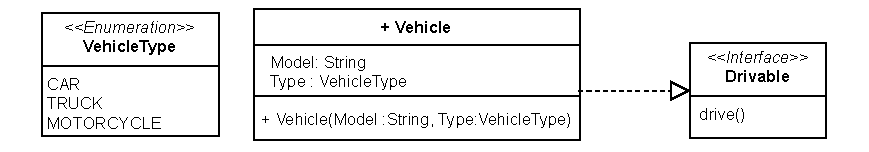
\includegraphics[width=\textwidth]{Chapters/Diagram/OOP/EX1/ex1.drawio.pdf}

\begin{prettyBox}{Note}{red}
When class implements an interface there is no need to list the implemented methods
\end{prettyBox}


\subsubsection*{\underline{Java Code :}}

\subsubsection*{\underline{Vehicle Class :}}
\lstinputlisting[style=javaStyle]{Chapters/JAVA/EX1/Vehicle.java}

\newpage
\subsubsection*{\underline{VehicleType Enumeration :}}
\lstinputlisting[style=javaStyle]{Chapters/JAVA/EX1/VehicleType.java}
\subsubsection*{\underline{Drivable Interface :}}
\lstinputlisting[style=javaStyle]{Chapters/JAVA/EX1/Drivable.java}


\subsubsection{Cardinalities}

\begin{prettyBox}{Cardinality}{mypur}
Cardinality in UML defines the number of instances of one class that can or must be associated with an instance of another class. It helps indicate the number of objects involved in aggregation , association, compostion relation.\\[0.25cm]
\textbf{How to Read Cardinality:}\\[0.15cm]
Cardinality is represented by numbers near a class, The format is typically `min..max` , so if there is association
between student and teacher , card near teacher would be how many instance of student for 1 teacher , and cardinality near
student class would be how many instance of teacher for 1 student\\[0.25cm]  
\textbf{Examples:}
\begin{itemize}
    \item `1` near the class means \textbf{exactly one instance}. 
    \item `0..1` means \textbf{zero or one instance}.
    \item `0..*` means \textbf{zero or more instances} (unlimited).
    \item `1..*` means \textbf{one or more instances} (unlimited).
\end{itemize}


\end{prettyBox}

\subsubsection{Relations Between Class}


\subsubsection*{Simple Relation(Association)}
\begin{prettyBox}{Association}{mypur}
Association is represented as a solid line between classes. It indicates that one class references another. There are several types of associations:
\begin{itemize}
    \item \textbf{Reflexive Association}: A class references itself.
    \item \textbf{Unidirectional Association}: One class references another class, but the reverse is not true.
    \item \textbf{Bidirectional Association}: Two classes reference each other.
    \item \textbf{N-ary Association}: An association involving more than two classes.
    \item \textbf{Association Class}: The association between classes is created through separate class that references the participating classes and may include additional attributes or behaviors ,  it is represented by dashed line 
connecting between association class and solid line association.
\end{itemize}
\end{prettyBox}

\vspace{0.25cm}

\begin{prettyBox}{Note}{red}
There is no need to explicitly list references of the other classes in the class association
because it is implicitly implied
\end{prettyBox}

\subsubsection*{\underline{Example :}}

\subsubsection*{\underline{Reflexive Association}}
Employee class that references itself to have a supervisor or manager , so an employee is managed by one manager , and a manager manages many employees 

\subsubsection*{\underline{UML}}

\begin{center}
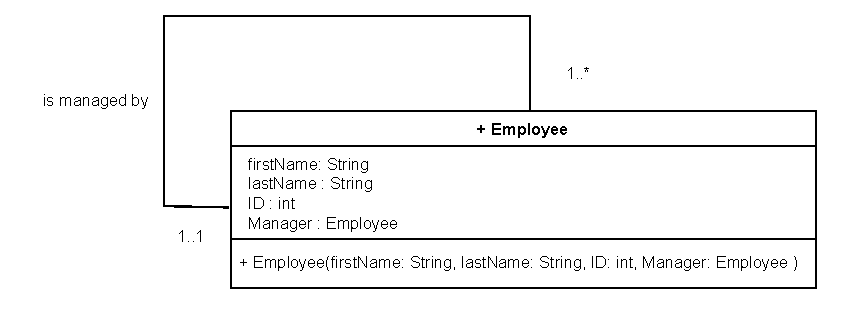
\includegraphics[width=0.65\textwidth]{Chapters/Diagram/OOP/EX2/ex2.a.drawio.pdf}
\end{center}


\subsubsection*{\underline{Employee Class}}
\lstinputlisting[style=javaStyle]{Chapters/JAVA/EX2/A/Employee.java}


\subsubsection*{\underline{Uni-direction Association}}
\subsubsection*{\underline{UML}}

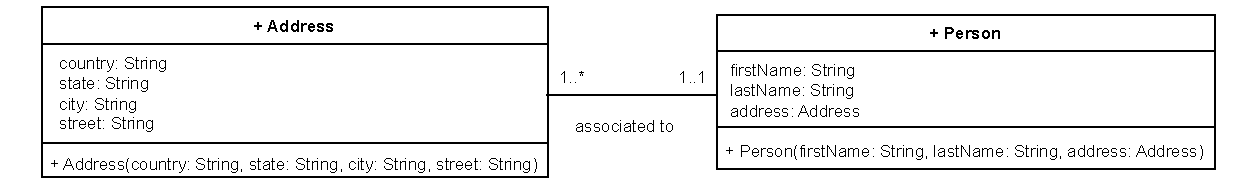
\includegraphics[width=\textwidth]{Chapters/Diagram/OOP/EX2/ex2.b.drawio.pdf}

\subsubsection*{\underline{Java Code}}

\subsubsection*{\underline{Person Class}}
\lstinputlisting[style=javaStyle]{Chapters/JAVA/EX2/B/Person.java}

\newpage
\subsubsection*{\underline{Address Class}}
\lstinputlisting[style=javaStyle]{Chapters/JAVA/EX2/B/Address.java}

\subsubsection*{\underline{Bi-direction Association}}
\subsubsection*{\underline{UML}}

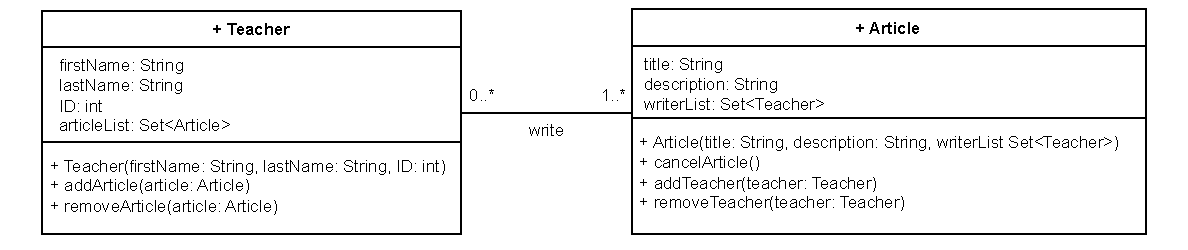
\includegraphics[width=\textwidth]{Chapters/Diagram/OOP/EX2/ex2.c.drawio.pdf}

\subsubsection*{\underline{Java Code}}

\vspace{-0.2cm}
\subsubsection*{\underline{Teacher Class}}

\vspace{-0.2cm}
\lstinputlisting[style=javaStyle]{Chapters/JAVA/EX2/C/Teacher.java}

\subsubsection*{\underline{Article Class}}
\lstinputlisting[style=javaStyle]{Chapters/JAVA/EX2/C/Article.java}



\subsubsection*{\underline{Association Class}}
\subsubsection*{\underline{UML}}


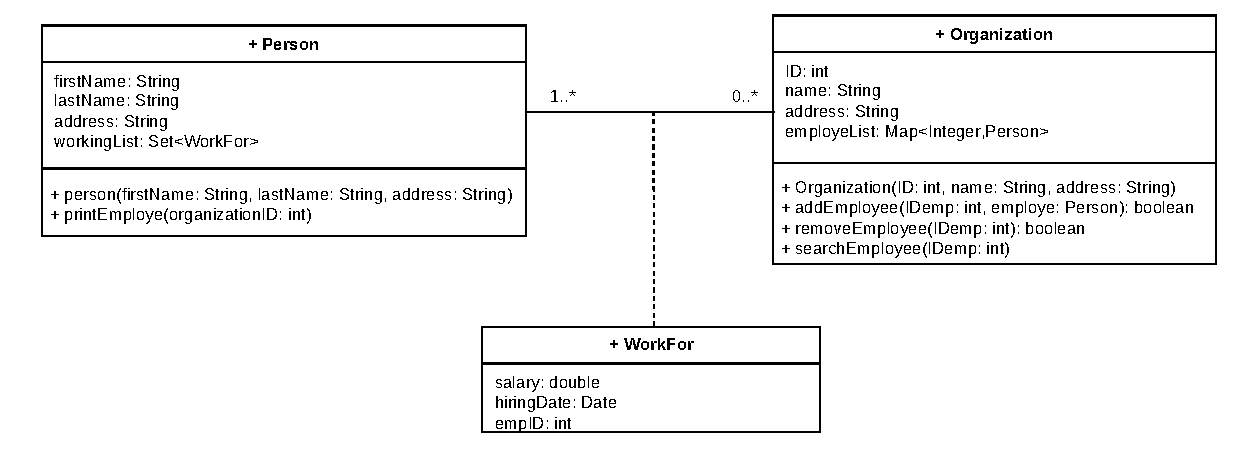
\includegraphics[width=\textwidth]{Chapters/Diagram/OOP/EX2/ex2.d.drawio.pdf}

\subsubsection*{\underline{Person Class}}

\lstinputlisting[style=javaStyle]{Chapters/JAVA/EX2/D/Person.java}

\subsubsection*{\underline{Organization Class}}
\lstinputlisting[style=javaStyle]{Chapters/JAVA/EX2/D/Organization.java}

\newpage
\subsubsection*{\underline{WorkFor Class}}
\lstinputlisting[style=javaStyle]{Chapters/JAVA/EX2/D/WorkFor.java}


\subsubsection*{\underline{3-ary Association}}
\subsubsection*{\underline{UML}}

\begin{center}
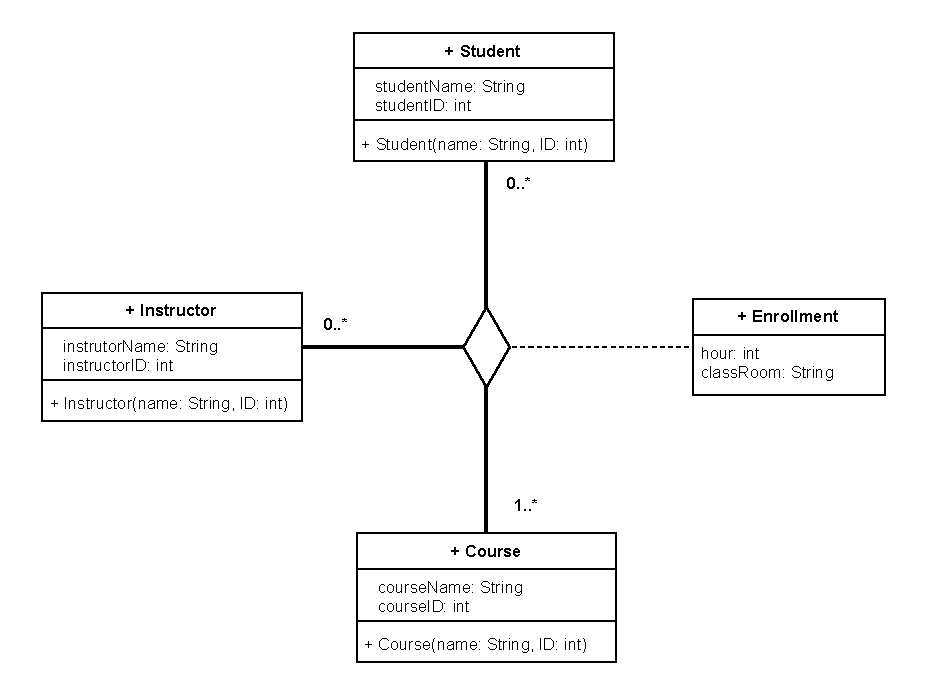
\includegraphics[width=0.7\textwidth]{Chapters/Diagram/OOP/EX2/ex2.e.drawio.pdf}
\end{center}


\subsubsection*{\underline{Java Code}}

\subsubsection*{\underline{Course Class}}

\lstinputlisting[style=javaStyle]{Chapters/JAVA/EX2/E/Course.java}

\newpage
\subsubsection*{\underline{Instructor Class}}
\lstinputlisting[style=javaStyle]{Chapters/JAVA/EX2/E/Instructor.java}

\subsubsection*{\underline{Student Class}}
\lstinputlisting[style=javaStyle]{Chapters/JAVA/EX2/E/Student.java}


\subsubsection*{\underline{Enrollment Class}}
\lstinputlisting[style=javaStyle]{Chapters/JAVA/EX2/E/Enrollment.java}

\subsubsection*{Dependency}

\begin{prettyBox}{Dependency}{mypur}
A dependency is represented by a dashed line with an arrow pointing to the \textbf{provider class}. It indicates a \textbf{temporary relationship} between two classes, where one class relies on the other to perform a specific function or operation. The types of dependency include:
\begin{itemize}
    \item \textbf{Method Call:} One class calls a method of another class without retaining a permanent reference.
    \item \textbf{Object Usage:} One class temporarily interacts with an object of another class, either as:
    \begin{itemize}
        \item \textbf{method parameter}.
        \item \textbf{return type}.
    \end{itemize}
\end{itemize}
\end{prettyBox}

\begin{prettyBox}{Difference Between Association \& Dependency}{red}
A dependency is a \textbf{weaker relationship} compared to an association. Unlike an association, which represents a \textbf{permanent structural relationship} (e.g., an instance variable), a dependency represents a \textbf{temporary interaction}. 

In a dependency:
\begin{itemize}
    \item The referenced object is used only temporarily and is eligible for garbage collection once the interaction ends.
    \item The classes are loosely coupled, meaning changes to one class have a lower impact on the other.
\end{itemize}

In contrast, an \textbf{association} involves a permanent reference to another class that exists as long as the object itself exists.
\end{prettyBox}


\subsubsection*{\underline{Method Call}}

\subsubsection*{\underline{UML}}
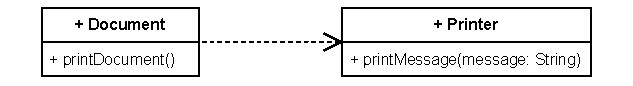
\includegraphics[width=\textwidth]{Chapters/Diagram/OOP/EX3/ex3.a.drawio.pdf}


\subsubsection*{\underline{Printer Class}}
\lstinputlisting[style=javaStyle]{Chapters/JAVA/EX3/A/Printer.java}

\subsubsection*{\underline{Document Class}}
\lstinputlisting[style=javaStyle]{Chapters/JAVA/EX3/A/Document.java}


\subsubsection*{\underline{Object Parameter In Method}}
\subsubsection*{\underline{UML}}
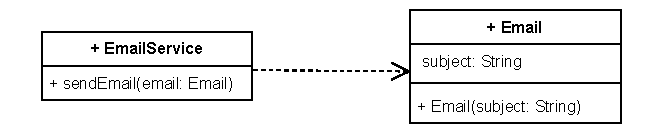
\includegraphics[width=\textwidth]{Chapters/Diagram/OOP/EX3/ex3.b.drawio.pdf}

\subsubsection*{\underline{Email Class}}
\lstinputlisting[style=javaStyle]{Chapters/JAVA/EX3/B/Email.java}

\subsubsection*{\underline{EmailService Class}}
\lstinputlisting[style=javaStyle]{Chapters/JAVA/EX3/B/EmailService.java}


\subsubsection*{\underline{Return Type Of A Method}}
\subsubsection*{\underline{UML}}
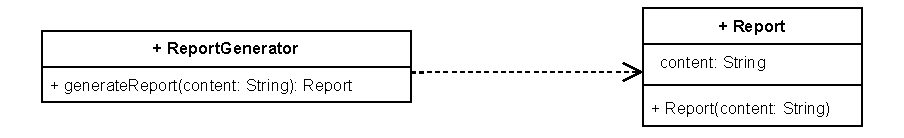
\includegraphics[width=\textwidth]{Chapters/Diagram/OOP/EX3/ex3.c.drawio.pdf}

\subsubsection*{\underline{Report Class}}
\lstinputlisting[style=javaStyle]{Chapters/JAVA/EX3/C/Report.java}

\subsubsection*{\underline{ReportGenerator Class}}
\lstinputlisting[style=javaStyle]{Chapters/JAVA/EX3/C/ReportGenerator.java}

\subsubsection*{Inheritance}

\begin{prettyBox}{Inheritance}{mypur}
Inheritance occurs when a class \textbf{extends} (inherits from) another class. It is represented in UML by a \textbf{solid line with a hollow triangle} at the end, pointing to the \textbf{parent class}.
\end{prettyBox}

\begin{prettyBox}{Note}{red}
Since child inherites all attributes and methods of parent class \textbf{we don't have to explicitly list them unless a method was ovveriden or changed visbility of an attribute}
\end{prettyBox}

\subsubsection*{\underline{Example}}

\subsubsection*{\underline{UML}}

\begin{center}
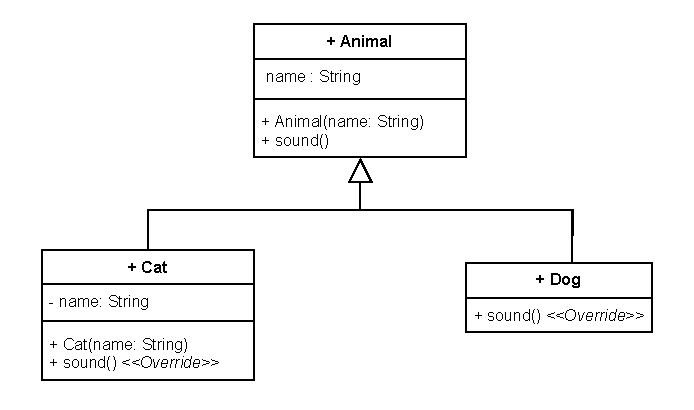
\includegraphics[width=0.6\textwidth]{Chapters/Diagram/OOP/EX4/ex4.drawio.pdf}
\end{center}


\subsubsection*{\underline{Animal Class}}
\lstinputlisting[style=javaStyle]{Chapters/JAVA/EX4/Animal.java}

\subsubsection*{\underline{Cat Class}}
\lstinputlisting[style=javaStyle]{Chapters/JAVA/EX4/Cat.java}

\subsubsection*{\underline{Dog Class}}
\lstinputlisting[style=javaStyle]{Chapters/JAVA/EX4/Dog.java}

\subsubsection*{Aggregation}

\begin{prettyBox}{Aggregation}{mypur}
Aggregation is a stronger relationship than association. It involves two classes: a whole class and a part class. The whole class references the part class, but the part class exists independently of the whole class. The part class is unaware of the whole class. Even if the whole class is destroyed by the garbage collector, the part class continues to exist.
\end{prettyBox}

\subsubsection*{\underline{Example}}

\subsubsection*{\underline{UML}}

\begin{center}
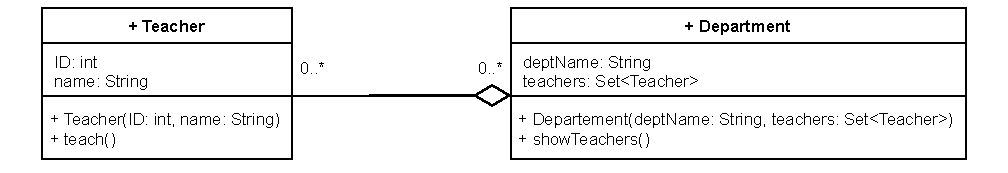
\includegraphics[width=0.9\textwidth]{Chapters/Diagram/OOP/EX5/ex5.drawio.pdf}
\end{center}


\subsubsection*{\underline{Teacher Class}}
\lstinputlisting[style=javaStyle]{Chapters/JAVA/EX5/Teacher.java}

\subsubsection*{\underline{Department Class}}
\lstinputlisting[style=javaStyle]{Chapters/JAVA/EX5/Department.java}

\subsubsection*{Composition}

\begin{prettyBox}{Composition}{mypur}
Composition is a stronger relationship than aggregation. In composition, when the whole class is deleted, the part class is also deleted, as the part is tightly bound and dependent to the whole.
\end{prettyBox}

\subsubsection*{\underline{Example}}

\subsubsection*{\underline{UML}}

\begin{center}
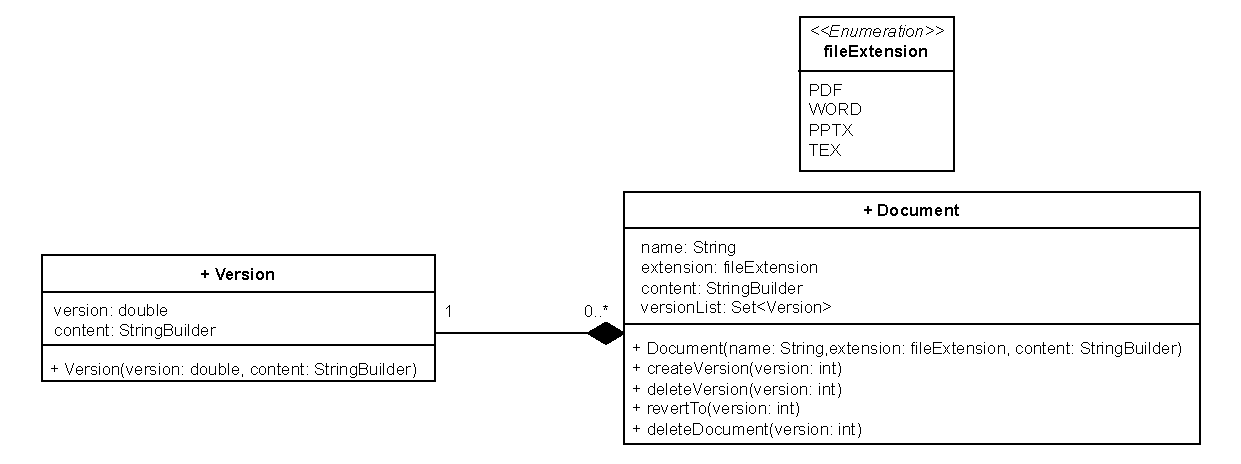
\includegraphics[width=0.9\textwidth]{Chapters/Diagram/OOP/EX6/ex6.drawio.pdf}
\end{center}

\subsubsection*{\underline{Version Class}}
\lstinputlisting[style=javaStyle]{Chapters/JAVA/EX6/Version.java}

\subsubsection*{\underline{fileExtension Enumeration}}
\lstinputlisting[style=javaStyle]{Chapters/JAVA/EX6/FileExtension.java}

\newpage
\subsubsection*{\underline{Document Class}}
\lstinputlisting[style=javaStyle]{Chapters/JAVA/EX6/Document.java}

\subsection{Summary}

\subsubsection*{\underline{Enumeration}}
\begin{center}
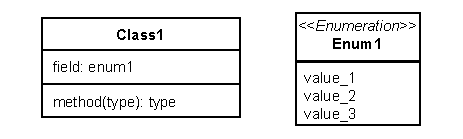
\includegraphics[width=0.6\textwidth]{Chapters/Diagram/OOP/Sum/Enum/enum.drawio.pdf}
\end{center}

\subsubsection*{\underline{Interface}}
\begin{center}
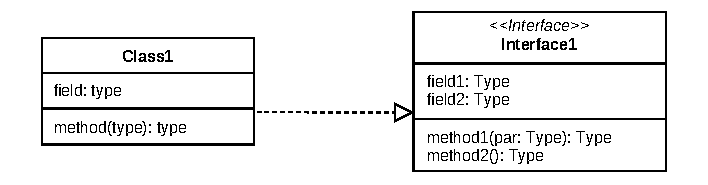
\includegraphics[width=0.8\textwidth]{Chapters/Diagram/OOP/Sum/Inter/inte.drawio.pdf}
\end{center}

\subsubsection*{\underline{Reflexive Association}}
\begin{center}
    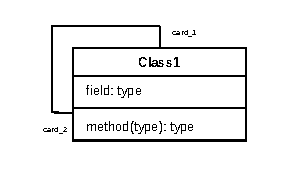
\includegraphics[width=0.4\textwidth]{Chapters/Diagram/OOP/Sum/reflexiveAssoc/selfassoc.drawio.pdf}
\end{center}

\subsubsection*{\underline{Simple Association}}

\begin{center}
   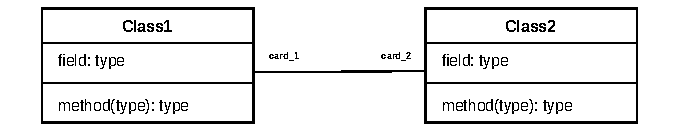
\includegraphics[width=0.75\textwidth]{Chapters/Diagram/OOP/Sum/SAssoc/simpleassoc.drawio.pdf}
\end{center}

\subsubsection*{\underline{N-ary Association}}

\begin{center}
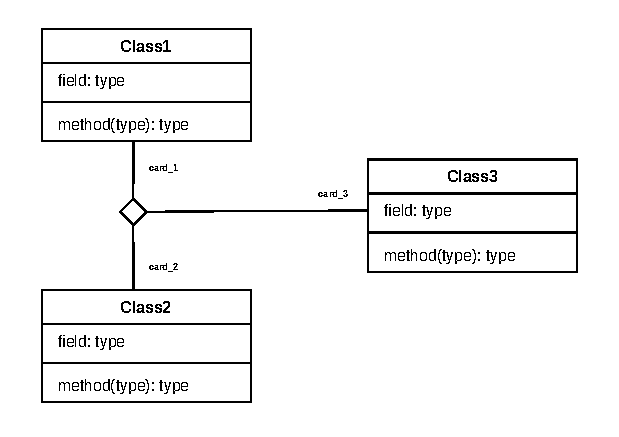
\includegraphics[width=0.65\textwidth]{Chapters/Diagram/OOP/Sum/NaryAssoc/naryassoc.drawio.pdf}
\end{center}

\subsubsection*{\underline{Class Association}}

\begin{center}
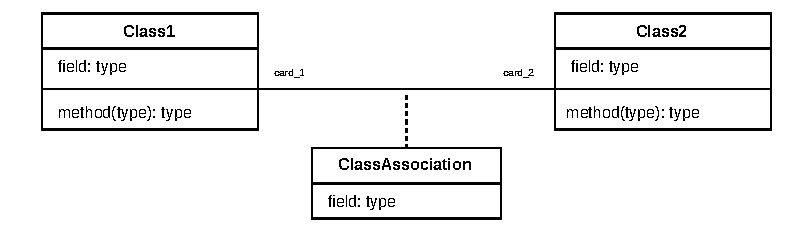
\includegraphics[width=0.75\textwidth]{Chapters/Diagram/OOP/Sum/Class Association/classassoc.drawio.pdf}
\end{center}

\subsubsection*{\underline{Dependency}}

\begin{center}
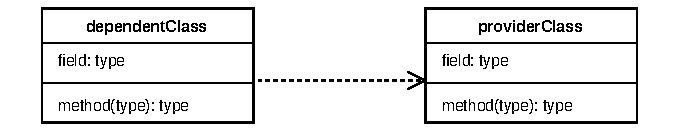
\includegraphics[width=0.75\textwidth]{Chapters/Diagram/OOP/Sum/Depend/depend.drawio.pdf}
\end{center}

\subsubsection*{\underline{Inheritance}}

\begin{center}
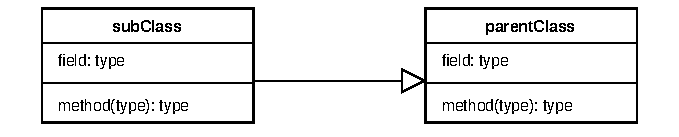
\includegraphics[width=0.75\textwidth]{Chapters/Diagram/OOP/Sum/Inhe/inherit.drawio.pdf}
\end{center}

\subsubsection*{\underline{Aggregation}}

\begin{center}
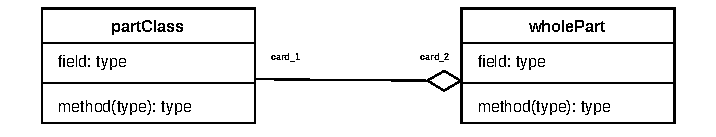
\includegraphics[width=0.75\textwidth]{Chapters/Diagram/OOP/Sum/Aggrega/aggrega.drawio.pdf}
\end{center}

\subsubsection*{\underline{Composition}}

\begin{center}
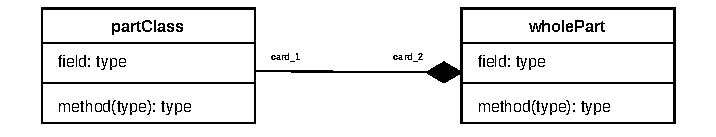
\includegraphics[width=0.75\textwidth]{Chapters/Diagram/OOP/Sum/Composition/composition.drawio.pdf}
\end{center}
